\documentclass{article}

\title{Simple Regression Analysis}
\author{Bret Hart}
\date{\today}
\usepackage{amsmath}
\usepackage{graphicx}

\usepackage{Sweave}
\begin{document}
\input{lab9-concordance}
\maketitle






\begin{abstract}

The aim of this report is to reproduce the main graphical and statistical results displayed in chapter 3.1, \textit{Simple Linear Regression}, of \textbf{An Introduction to Statistical Learning}. Referred to as \textbf{ISLR}, the textbook is a manifesto to Machine Learning and Linear Models, teaching the material in an approachable yet sophisticated way. In addition, the data used to generate all of the graphs, plots, etc. in the text are freely available - advancing and standing for the tenants of reproducible research, even in a textbook. We seek to create an automated repository which can recreate the findings that they display, using the same data set.

\end{abstract}

\section*{Introduction}

The data set which we are studying is an Advertising data set - it is a collection of money spent in 200 different markets on Advertising and each market's corresponding Sales figures. While the data also includes information on Newspaper and Radio advertisement, for the purpose of this project, we are going to focus on Television advertisement expenditure. We would like to determine whether there is a meaningful, significant relationship between TV advertisement and Sales, and, using these results, predict future Sales figures based on amounts of Advertisement expenditure. Ultimately, we would like to make sophisticated, informed decisions on how to form an Advertising plan in the future. We want to model this relationship effectively and correctly, and use the model to predict future sales and create a profitable Sales plan.


\section*{Data}

More specifically, the Advertising data sets contains \textbf{Sales} (in thousands of units) of a particular product in 200 different markets, supplemented by advertising budgets (in thousands of dollars) for the products in three different forms of media: \textbf{TV}, \textbf{Radio}, and \textbf{Newspaper}. For this, however, we are going to focus primarily on the relationship between \textbf{TV} and \textbf{Sales}, for the purposes of specifically reproducing the figures and findings in \textbf{ISLR}.


\section*{Methodology}

As stated previously, we are focusing on the advertising medium of \textbf{TV} and its relationship with \textbf{Sales}. To do this, we will assume and use the simple linear model:

\begin{equation*}
\textbf{Sales} = \beta_0 + \beta_1 \textbf{TV}
\end{equation*}

To estimate the coefficients  $\beta_0$  and   $\beta_1$ we fit a regression model via the least squares criterion.



\section*{Results}

We estimate the regression coefficients via the least squares method in Table 1:






\begin{table}[ht]
\centering
\caption{Information about Regression Coefficients}
\begin{tabular}{rrrrr}
\hline
& Estimate & Std. Error & t value & Pr($>$$|$t$|$) \\
\hline
(Intercept) & 7.03 & 0.46 & 15.36 & 0.00 \\
TV & 0.05 & 0.00 & 17.67 & 0.00 \\
\hline
\end{tabular}
\end{table}


Some statistics of the least squares model are presented in Table 2:



%<<MyLaTeXT1, echo = FALSE>>=
%xtable(x.stats)
%@


\begin{table}[ht]
\centering
\caption{Regression Statistics}
\begin{tabular}{rll}
\hline
& Statistic & Value \\
\hline
1 & RSE & 3.26 \\
2 & RSS & 2102.53 \\
3 & R2 & 0.61 \\
4 & F-stat & 312.14 \\
\hline
\end{tabular}
\end{table}



Lastly, here is the scatterplot of the mapped Television vs. Sales values, with fitted regression line:

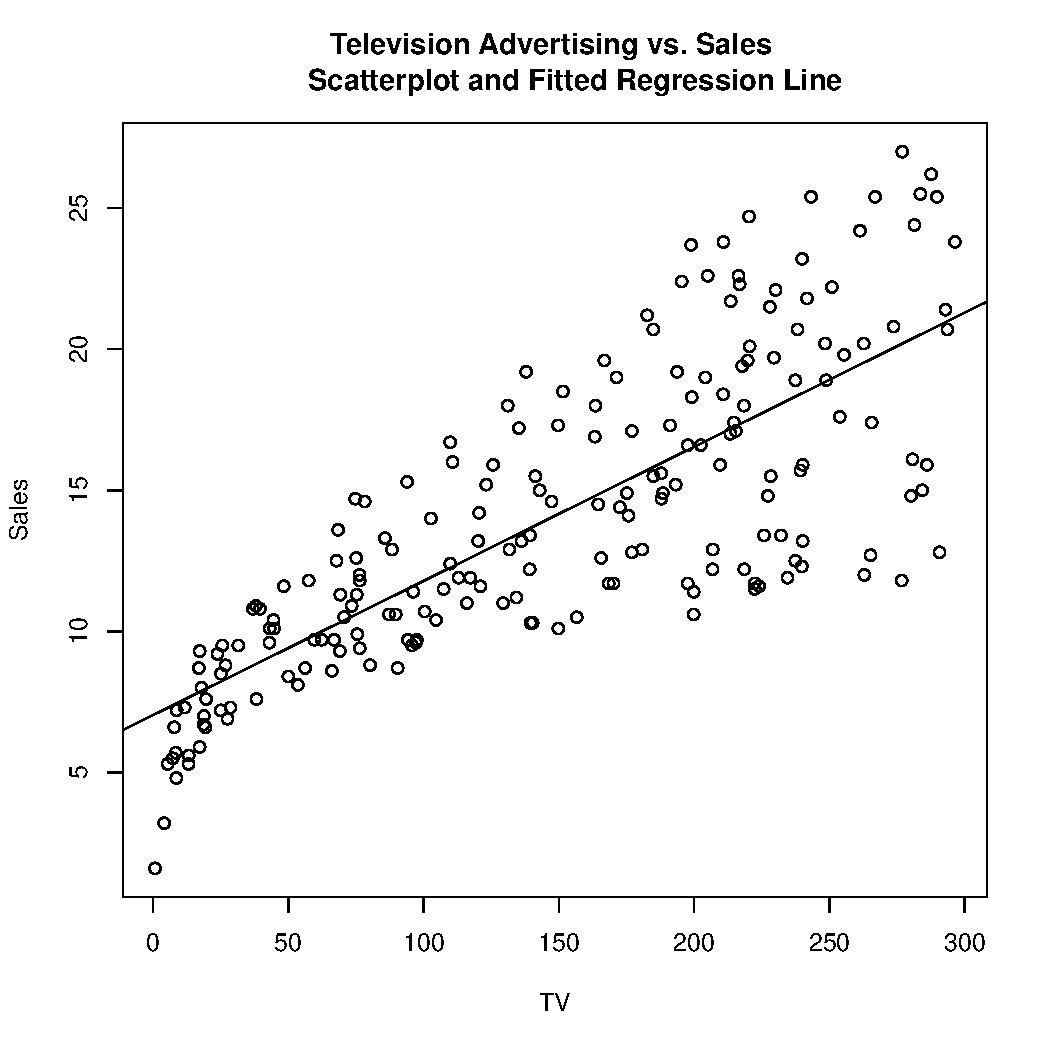
\includegraphics[]{scatterplot-tv-sales.pdf}




\section*{Conclusions}

Based on the extremely high t-value for \textbf{TV}, it can be surmised that, when other variables are not accounted for, \textbf{TV} advertisement has a significantly large chance of having an effect on \textbf{Sales}. Of course, a conclusion based solely on a t-statistic in a vacuum will be innacurate, as the other variables (\textbf{Newspaper}, \textbf{Radio}) likely influence the markets that \textbf{TV} advertising is taking place in to a substantial degree. In addition to the t-statistic, the F-statistic is extremely large as well, but it holds less meaning when there are not multple predictors being matched to a dependent variable. Although its relevancy is questionable, having a significant F-statistic surely helps.  


Having a low RSE and realistically substantial R2 value, though, add a good deal of certainty to the reasonability of a statistically relevant fit. While neither statistics are showcasing an extremely close fit, they suggest good things about the goodness of fit, the correlation between \textbf{TV} and \textbf{Sales}, and substantially bolster the argument that \textbf{TV} is an important predictor in determining product sales in a market.  


Some interesting observations are that, as TV advertising increases, Sales becomes more variable, in a very observable fashion. Perhaps these markets have subsequently less (or more) advertisement spending in the other mediums, influenced by the increase in TV spending, which leads to these more wild and unpredictable Sales figures. Additionally, there seem to be a pretty equal number of points above and below the line, but a general trend upwards. This is no detriment to a linear model, as the general upward trend is far more signifcant than spread out values.   


Ultimately, increasing \textbf{TV} spending seems to have a statistically significant effect on an increase in Sales, but a realistic spending model will take into account how much these product sales really mean in response to a significant but not very positive relationship. The coefficient of \textbf{TV} in the regression line is pretty small, so although advertising does seem to have a net positive effect, there is definitely going to be a drop-off in how lucrative increasing expenditures will be past a certain point. Eventually advertising spending will overshadow actual sales revenue, so the acknowledgement of a significant but not very positive relationship can help color marketing decisions in the future. Additionally, it would be wise to start measuring the effects of the other predictors in tandem with \textbf{TV}, as these numbers are surely not telling the whole story.




\end{document}

